% Created by tikzDevice version 0.12.6 on 2025-04-16 12:13:28
% !TEX encoding = UTF-8 Unicode
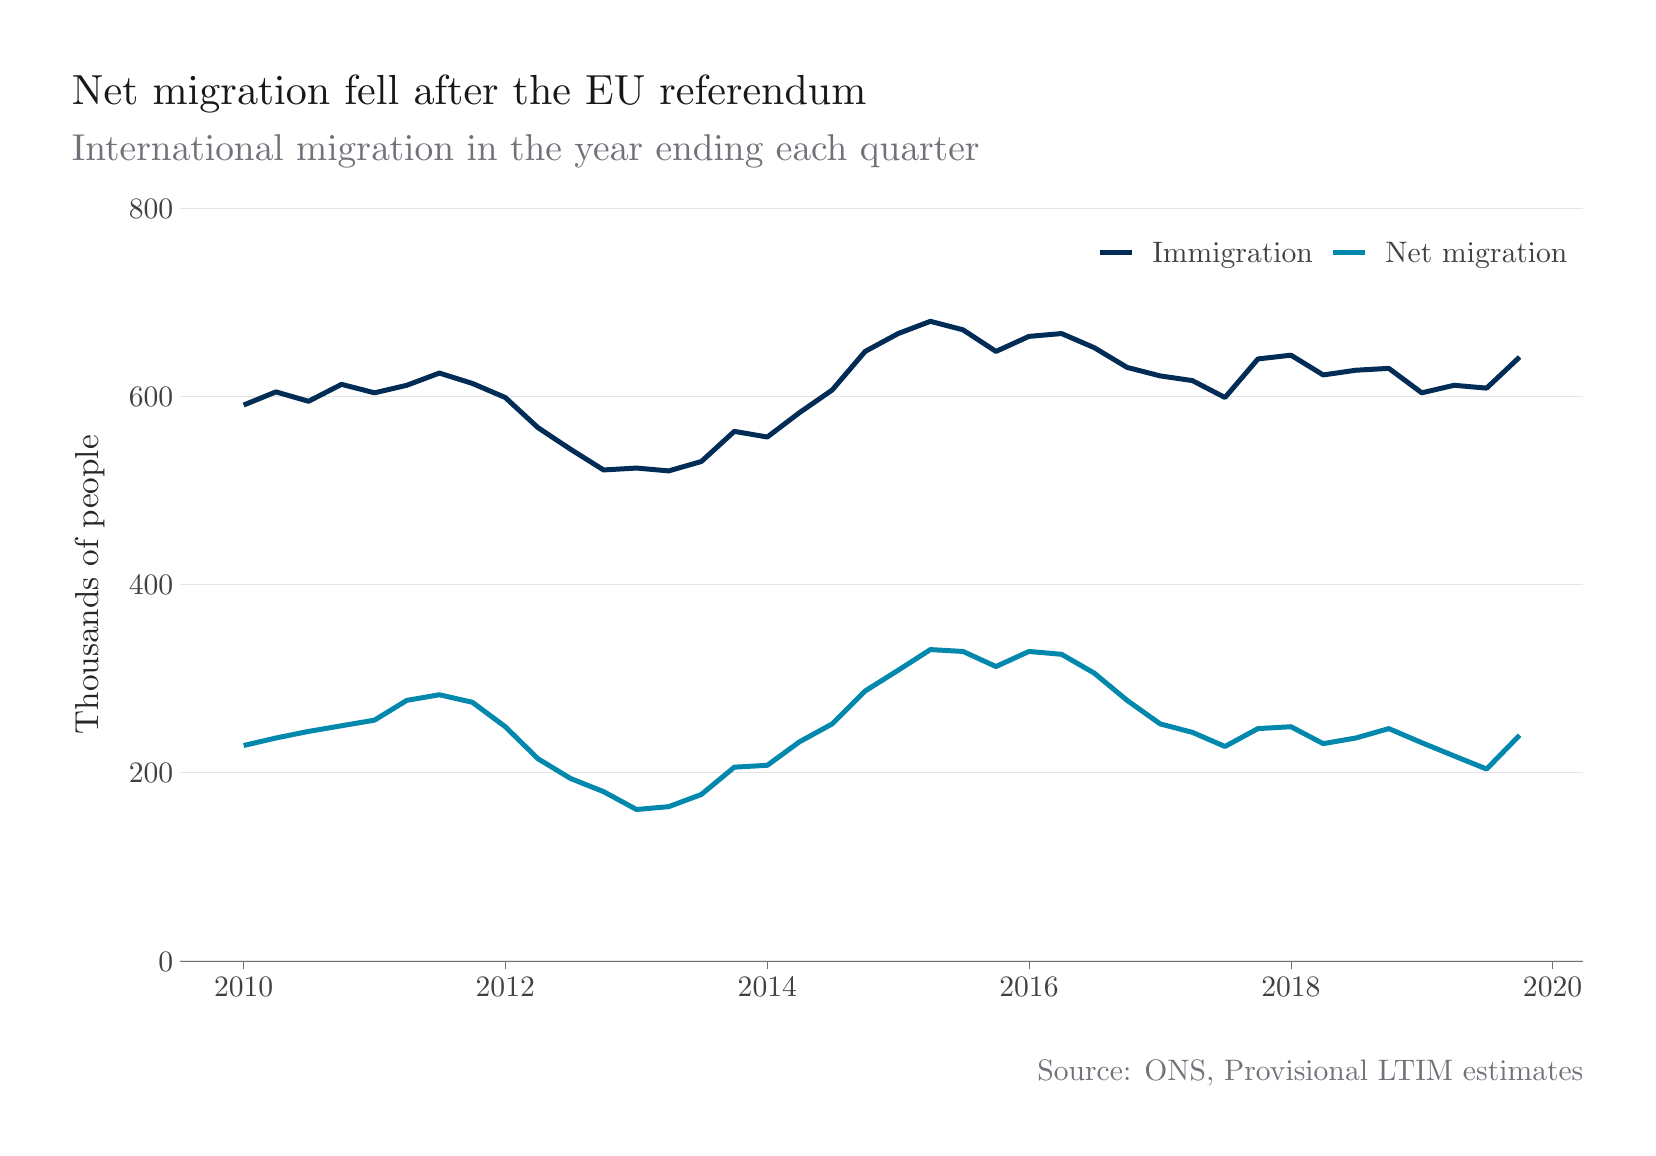
\begin{tikzpicture}[x=1pt,y=1pt]
\definecolor{fillColor}{RGB}{255,255,255}
\path[use as bounding box,fill=fillColor] (0,0) rectangle (578.16,397.48);
\begin{scope}
\path[clip] (  0.00,  0.00) rectangle (578.16,397.48);
\definecolor{drawColor}{RGB}{255,255,255}

\path[draw=drawColor,line width= 0.6pt,line join=round,line cap=round,fill=fillColor] (  0.00,  0.00) rectangle (578.16,397.48);
\end{scope}
\begin{scope}
\path[clip] ( 55.00, 60.25) rectangle (562.16,332.15);
\definecolor{drawColor}{RGB}{255,255,255}
\definecolor{fillColor}{RGB}{255,255,255}

\path[draw=drawColor,line width= 0.6pt,line join=round,line cap=round,fill=fillColor] ( 55.00, 60.25) rectangle (562.16,332.15);
\definecolor{drawColor}{RGB}{228,228,231}

\path[draw=drawColor,line width= 0.4pt,line join=round] ( 55.00, 60.25) --
	(562.16, 60.25);

\path[draw=drawColor,line width= 0.4pt,line join=round] ( 55.00,128.22) --
	(562.16,128.22);

\path[draw=drawColor,line width= 0.4pt,line join=round] ( 55.00,196.20) --
	(562.16,196.20);

\path[draw=drawColor,line width= 0.4pt,line join=round] ( 55.00,264.17) --
	(562.16,264.17);

\path[draw=drawColor,line width= 0.4pt,line join=round] ( 55.00,332.15) --
	(562.16,332.15);
\definecolor{drawColor}{RGB}{0,44,85}

\path[draw=drawColor,line width= 1.8pt,line join=round] ( 78.05,261.11) --
	( 89.71,265.87) --
	(101.49,262.47) --
	(113.41,268.59) --
	(125.32,265.53) --
	(136.98,268.25) --
	(148.76,272.67) --
	(160.68,268.93) --
	(172.59,263.83) --
	(184.38,252.96) --
	(196.16,245.14) --
	(208.08,237.66) --
	(219.99,238.34) --
	(231.65,237.32) --
	(243.44,240.72) --
	(255.35,251.60) --
	(267.27,249.56) --
	(278.92,258.39) --
	(290.71,266.55) --
	(302.62,280.49) --
	(314.54,286.94) --
	(326.19,291.36) --
	(337.98,288.30) --
	(349.89,280.49) --
	(361.81,285.92) --
	(373.59,286.94) --
	(385.38,281.85) --
	(397.29,274.71) --
	(409.21,271.65) --
	(420.86,269.95) --
	(432.65,263.83) --
	(444.56,277.77) --
	(456.48,279.13) --
	(468.14,271.99) --
	(479.92,273.69) --
	(491.84,274.37) --
	(503.75,265.53) --
	(515.41,268.25) --
	(527.19,267.23) --
	(539.11,278.45);
\definecolor{drawColor}{RGB}{1,136,172}

\path[draw=drawColor,line width= 1.8pt,line join=round] ( 78.05,138.08) --
	( 89.71,140.80) --
	(101.49,143.18) --
	(113.41,145.22) --
	(125.32,147.25) --
	(136.98,154.39) --
	(148.76,156.43) --
	(160.68,153.71) --
	(172.59,144.88) --
	(184.38,133.32) --
	(196.16,126.18) --
	(208.08,121.42) --
	(219.99,114.97) --
	(231.65,115.99) --
	(243.44,120.40) --
	(255.35,130.26) --
	(267.27,130.94) --
	(278.92,139.44) --
	(290.71,145.90) --
	(302.62,157.79) --
	(314.54,165.27) --
	(326.19,172.75) --
	(337.98,172.07) --
	(349.89,166.63) --
	(361.81,172.07) --
	(373.59,171.05) --
	(385.38,164.25) --
	(397.29,154.39) --
	(409.21,145.90) --
	(420.86,142.84) --
	(432.65,137.74) --
	(444.56,144.20) --
	(456.48,144.88) --
	(468.14,138.76) --
	(479.92,140.80) --
	(491.84,144.20) --
	(503.75,139.10) --
	(515.41,134.34) --
	(527.19,129.58) --
	(539.11,141.82);
\end{scope}
\begin{scope}
\path[clip] (  0.00,  0.00) rectangle (578.16,397.48);
\definecolor{drawColor}{RGB}{63,63,70}

\node[text=drawColor,anchor=base east,inner sep=0pt, outer sep=0pt, scale=  1.07] at ( 52.60, 56.57) {0};

\node[text=drawColor,anchor=base east,inner sep=0pt, outer sep=0pt, scale=  1.07] at ( 52.60,124.55) {200};

\node[text=drawColor,anchor=base east,inner sep=0pt, outer sep=0pt, scale=  1.07] at ( 52.60,192.52) {400};

\node[text=drawColor,anchor=base east,inner sep=0pt, outer sep=0pt, scale=  1.07] at ( 52.60,260.50) {600};

\node[text=drawColor,anchor=base east,inner sep=0pt, outer sep=0pt, scale=  1.07] at ( 52.60,328.47) {800};
\end{scope}
\begin{scope}
\path[clip] (  0.00,  0.00) rectangle (578.16,397.48);
\definecolor{drawColor}{RGB}{113,113,122}

\path[draw=drawColor,line width= 0.3pt,line join=round] ( 55.00, 60.25) --
	(562.16, 60.25);
\end{scope}
\begin{scope}
\path[clip] (  0.00,  0.00) rectangle (578.16,397.48);
\definecolor{drawColor}{RGB}{113,113,122}

\path[draw=drawColor,line width= 0.3pt,line join=round] ( 78.05, 57.25) --
	( 78.05, 60.25);

\path[draw=drawColor,line width= 0.3pt,line join=round] (172.59, 57.25) --
	(172.59, 60.25);

\path[draw=drawColor,line width= 0.3pt,line join=round] (267.27, 57.25) --
	(267.27, 60.25);

\path[draw=drawColor,line width= 0.3pt,line join=round] (361.81, 57.25) --
	(361.81, 60.25);

\path[draw=drawColor,line width= 0.3pt,line join=round] (456.48, 57.25) --
	(456.48, 60.25);

\path[draw=drawColor,line width= 0.3pt,line join=round] (551.02, 57.25) --
	(551.02, 60.25);
\end{scope}
\begin{scope}
\path[clip] (  0.00,  0.00) rectangle (578.16,397.48);
\definecolor{drawColor}{RGB}{63,63,70}

\node[text=drawColor,anchor=base,inner sep=0pt, outer sep=0pt, scale=  1.07] at ( 78.05, 47.50) {2010};

\node[text=drawColor,anchor=base,inner sep=0pt, outer sep=0pt, scale=  1.07] at (172.59, 47.50) {2012};

\node[text=drawColor,anchor=base,inner sep=0pt, outer sep=0pt, scale=  1.07] at (267.27, 47.50) {2014};

\node[text=drawColor,anchor=base,inner sep=0pt, outer sep=0pt, scale=  1.07] at (361.81, 47.50) {2016};

\node[text=drawColor,anchor=base,inner sep=0pt, outer sep=0pt, scale=  1.07] at (456.48, 47.50) {2018};

\node[text=drawColor,anchor=base,inner sep=0pt, outer sep=0pt, scale=  1.07] at (551.02, 47.50) {2020};
\end{scope}
\begin{scope}
\path[clip] (  0.00,  0.00) rectangle (578.16,397.48);
\definecolor{drawColor}{RGB}{39,39,42}

\node[text=drawColor,rotate= 90.00,anchor=base,inner sep=0pt, outer sep=0pt, scale=  1.20] at ( 25.43,196.20) {Thousands of people};
\end{scope}
\begin{scope}
\path[clip] (  0.00,  0.00) rectangle (578.16,397.48);
\definecolor{drawColor}{RGB}{255,255,255}
\definecolor{fillColor}{RGB}{255,255,255}

\path[draw=drawColor,line width= 0.6pt,line join=round,line cap=round,fill=fillColor] (379.92,302.98) rectangle (562.16,329.43);
\end{scope}
\begin{scope}
\path[clip] (  0.00,  0.00) rectangle (578.16,397.48);
\definecolor{drawColor}{RGB}{255,255,255}
\definecolor{fillColor}{RGB}{255,255,255}

\path[draw=drawColor,line width= 0.6pt,line join=round,line cap=round,fill=fillColor] (385.92,308.98) rectangle (400.38,323.43);
\definecolor{drawColor}{RGB}{0,44,85}

\path[draw=drawColor,line width= 1.8pt,line join=round] (387.37,316.20) -- (398.93,316.20);
\end{scope}
\begin{scope}
\path[clip] (  0.00,  0.00) rectangle (578.16,397.48);
\definecolor{drawColor}{RGB}{255,255,255}
\definecolor{fillColor}{RGB}{255,255,255}

\path[draw=drawColor,line width= 0.6pt,line join=round,line cap=round,fill=fillColor] (470.19,308.98) rectangle (484.64,323.43);
\definecolor{drawColor}{RGB}{1,136,172}

\path[draw=drawColor,line width= 1.8pt,line join=round] (471.64,316.20) -- (483.20,316.20);
\end{scope}
\begin{scope}
\path[clip] (  0.00,  0.00) rectangle (578.16,397.48);
\definecolor{drawColor}{RGB}{63,63,70}

\node[text=drawColor,anchor=base west,inner sep=0pt, outer sep=0pt, scale=  1.07] at (406.38,312.53) {Immigration};
\end{scope}
\begin{scope}
\path[clip] (  0.00,  0.00) rectangle (578.16,397.48);
\definecolor{drawColor}{RGB}{63,63,70}

\node[text=drawColor,anchor=base west,inner sep=0pt, outer sep=0pt, scale=  1.07] at (490.64,312.53) {Net migration};
\end{scope}
\begin{scope}
\path[clip] (  0.00,  0.00) rectangle (578.16,397.48);
\definecolor{drawColor}{RGB}{113,113,122}

\node[text=drawColor,anchor=base west,inner sep=0pt, outer sep=0pt, scale=  1.35] at ( 16.00,349.46) {International migration in the year ending each quarter};
\end{scope}
\begin{scope}
\path[clip] (  0.00,  0.00) rectangle (578.16,397.48);
\definecolor{drawColor}{RGB}{24,24,27}

\node[text=drawColor,anchor=base west,inner sep=0pt, outer sep=0pt, scale=  1.52] at ( 16.00,369.55) {Net migration fell after the EU referendum};
\end{scope}
\begin{scope}
\path[clip] (  0.00,  0.00) rectangle (578.16,397.48);
\definecolor{drawColor}{RGB}{113,113,122}

\node[text=drawColor,anchor=base east,inner sep=0pt, outer sep=0pt, scale=  1.07] at (562.16, 17.04) {Source: ONS, Provisional LTIM estimates};
\end{scope}
\end{tikzpicture}
